\section{Pasty pro hybridní integrované obvody}
-složení a význam jednotlivých složek, příprava a míchání past

\subsection{Složení a význam jednotlivých složek}
\textbf{Funkční složka:}
\begin{itemize}
\item vodivá
\item odporová
\item dielektrická
\item izolační
\end{itemize}

\textbf{Tavivová:}
\begin{itemize}
\item nízkotavné sklo
\end{itemize}

\textbf{Pojivová:}
\begin{itemize}
\item ředidla (terpineol)
\item organické složky (celuóza)
\item modifikátory
\end{itemize}

\subsubsection{Funkční}
\begin{itemize}
\item Kovy - vodivé vrstvy
\item Oxidy kovů - odporové vrstvy
\item Izolanty - dielektrické nebo krycí vrstvy
\end{itemize}

Jedná se o prášek zrnitosti cca od 1 - 10 $\mu$m(udávaný stření průměr kolem 5 $\mu$m).

Tvar částic může být velmi různorodý vzhledem k metodě
přípravy prášku (kuličky, vločky, oblé struktury) a to jak
krystalické, tak amorfní povahy.

Tvar, velikost a rozložení částic jsou velmi důležité pro
dosažení požadovaných parametrů vypálené vrstvy.

\subsubsection{Tavivová složka}

Používají se dva základní způsoby, které mohou být použity
samostatně nebo je možné je kombinovat. (skloviny, oxidy kovů)

\subsubsection*{Sklovina}
Mají relativně nízkou teplotu tavení cca 500 - 600 $^{\circ}$C. S těmito materiály jsou spojeny dva adhezní mechanismy:

\textbf{Chemická vazba}
\begin{itemize}
\item roztavená sklovina reaguje chemicky se sklovinou obsaženou v substrátu
\item je obecně více náchylná k poškození vlivem mechanického působení (namáhání /stresu)
\end{itemize}

\textbf{Fyzikální vazba}
\begin{itemize}
\item roztavená sklovina zatéká do (a kolem) nerovností substrátu, vtéká do
dutin a prohlubní a zachytává se na malých výběžcích substrátu
\item je náchylnější k degradaci tepelným zatěžováním / cyklováním
\end{itemize}

Celková přilnavost / adheze vrstvy je dána součtem těchto dvou faktorů.

Tato složka se skládá z nízkotavného skla např. B2O3 s přídavkem modifikátorů PbO, CdO, ZnO, Al2O3...

Vodivé vrstvy s touto tavivovou složkou jsou náchylné k vytlačování skloviny na povrch
vrstvy - s touto skutečností mohou být spojeny problémy s následnou montáží dalších
součástek a komponent, realizace vrstvového potenciometru, apod.

\subsubsection*{Oxidy kovů}

Používají se oxidy mědi (Cu) nebo kadmia (Cd), které se přidávají do pasty.

Tyto oxidy při výpalu reagují s atomy kyslíku na povrchu substrátu a vytváří tak
oxidovou vazbu - funkční vrstva / substrát.

Výpal se pohybuje typicky v rozmezí 950 - 1000 $^{\circ}$C. Tato skutečnost je z pohledu náročnosti a ekonomiky výroby vnímána problematicky (vysoká teplota výpalu = rychlé opotřebení pece = vysoké výrobní náklady).

\subsubsection*{Kombinace sklovin a oxidů kovů}

Jsou zde zastoupeny především oxidy ZnO a CaO, které interagují s kyslíkem již při
nižších teplotách,

Jejich vazba ovšem není tak pevná jako např. v případě oxidu mědi.

Je zde přidáno menší množství skloviny (než ve fritových pastách) k vylepšení
adheze vrstvy k substrátu.

Tento typ tavivové složky je známý jako “mix bonded system”.

Zahrnuje výhody obou předchozích systémů při menší vypalovací teplotě.

Vodivé vrstvy s touto tavivovou složkou jsou vhodné pro technologii kontaktování
pomocí mikrodrátků.

\subsubsection{Pojivová složka}

Jsou to v zásadě tixotropní kapaliny, které mají 2 účely:
\begin{itemize}
\item udržují pohromadě funkční a tavivovou složku v
suspenzi, dokud není vrstva vypálená
\item propůjčují pastě vhodné tiskové vlastnosti (sítotisk)
\end{itemize}

Obsahuje netěkavé organické sloučeniny, které vyhoří až na teplotách kolem 350 $^{\circ}$C.

Tato složka musí během výpalu shořet beze zbytků (uhlíkových), které by mohly
kontaminovat realizovanou vodivou vrstvu (zhoršení izolačních vlastností mezer, atd).

Samostatným tématem jsou pak vrstvy, které je třeba vypalovat v ochranné atmosféře,
která může obsahovat pouze stopové množství (ppm) zbytkového kyslíku. V těchto
případech totiž nemohou pojivové složky vyhořet, ale musejí se bezezbytku odpařit.

\subsubsection*{Rozpouštědla a ředidla}
 Organická pojiva jsou ve své přirozené formě pro potřebu depozice sítotiskem příliš hustá - toto
vyvolává potřebu použití rozpouštědel a ředidel.Těmito složkami tedy upravujeme finální tiskové paramtry pasty, kterou používánme pro
realiaci vrstvy.

 Ředidla a rozpouštědla jsou naopak od organických pojiv těkavá a vypařují se velmi rychle
již od teplot nad 100 $^{\circ}$C. Typickými materiály pro tento účel jsou terpineol nebo některé druhy složitých alkoholů, ve kterých se netěkavá složka rozpouští.

Je zde žádán velmi malý odpar při pokojové teplotě - důvodem je riziko vysychání a tím
změny viskozity např v průběhu tisku (doba zpracovatelnosti pasty).

Dodatečně se do rozpouštědel přidávají další modifikátory (změkčovadla / plastifikátory),
povrchově aktivní látky a další činidla, které modifikují tixotropní povahu past.

Všechny uvedené složky (funkční, tavivová a pojivová) se v TLV pastě mísí dohromady v
odpovídajícím poměru a propracovávají se spolu na tříválcovém mlýnku po dostatečně dlouhou
dobu, která zajistí důkladné promíchání s rovnoměrným rozložením jednotlivých složek v objemu
pasty.

\subsection{Příprava a míchání past}
Pasty jsou připravovány z práškových materiálů mícháním a roztíráním
(rozpracováním) těchto komponent s pojivem (např. terpineol),
které dodá příslušné pastě potřebnou viskozitu.

Materiálové kompozice jsou připravené
ve formě práškových frit, pokud možno
s co ne jdef inovanějším tvarem
jednotlivých částic (o průměru < 5 $\mu$m)
tak, aby byly zaručeny jak dobré tiskové
vlastnosti, tak také homogenita pasty při
jejím nanášení a následném výpalu

\begin{figure}[h]
   \begin{center}
     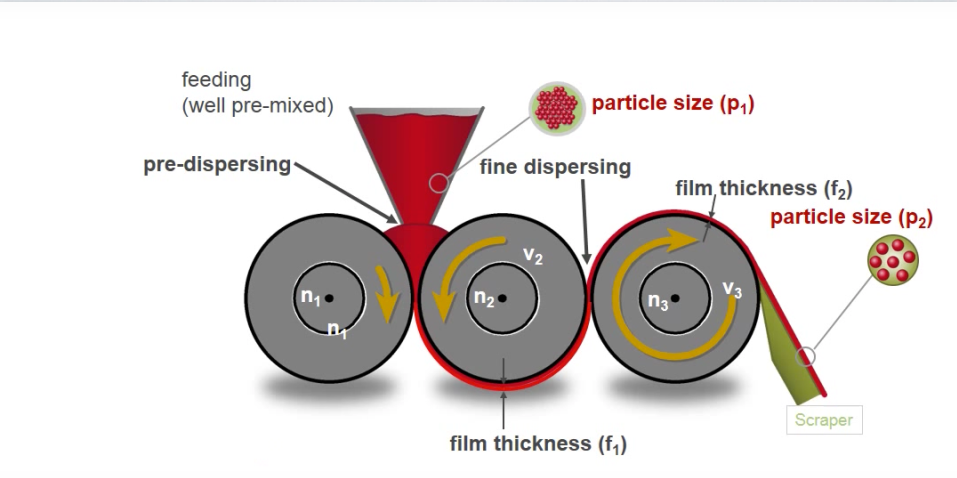
\includegraphics[scale=0.6]{images/mlyn.png}
   \end{center}
   \caption{Třívalcový mlýnek}
\end{figure}

\subsubsection{Rovnoměrnost rozložení jednotlivých složek v objemu pasty}
Velikost mezery definuje maximální velikost shluků materiálu, který projde.

Rozseparování částic shluků proběhne díky rozdílné rychlosti válců (střihová síla).

\begin{figure}[h]
   \begin{center}
     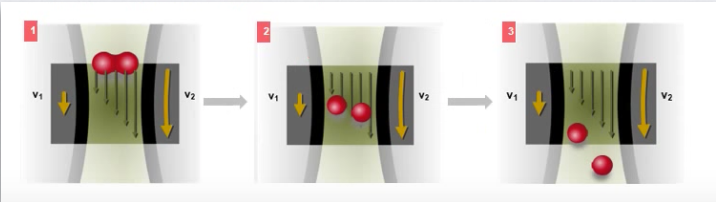
\includegraphics[scale=0.6]{images/separace.png}
   \end{center}
   \caption{Separace částic pasty}
\end{figure}
\newpage
Kvalita separace částic a homogennost jejich rozložení v pastě je dána
nastavením parametrů zařízení a počtem cyklů.

\begin{figure}[h]
   \begin{center}
     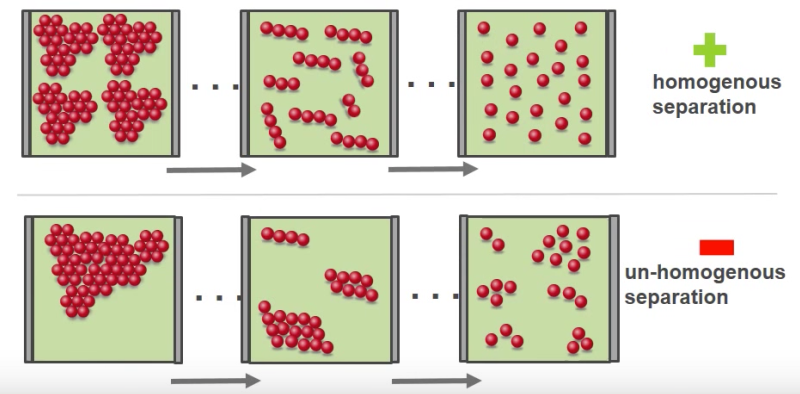
\includegraphics[scale=0.6]{images/hom.png}
   \end{center}
   \caption{Homogenní a nehomogenní pasta}
\end{figure}

























